\documentclass[10pt, aspectratio=169]{beamer}

\usepackage[utf8]{inputenc}
\usepackage[T1]{fontenc}
\usepackage{booktabs}
\usepackage{tikz}
\usetikzlibrary{positioning, arrows.meta, calc}

% ---------- bright theme ----------
\usetheme{Boadilla}
\definecolor{chessblue}{RGB}{0,105,217}
\definecolor{chesslight}{RGB}{230,240,255}
\setbeamercolor{structure}{fg=chessblue}
\setbeamercolor{frametitle}{bg=chessblue, fg=white}
\setbeamercolor{title}{fg=chessblue}
\setbeamercolor{palette primary}{bg=chessblue, fg=white}
\setbeamercolor{palette secondary}{bg=chessblue!80, fg=white}
\setbeamercolor{palette tertiary}{bg=chessblue!55, fg=white}
\setbeamercolor{block title}{bg=chessblue!12, fg=chessblue!55!black}
\setbeamercolor{block body}{bg=white}

\setbeamertemplate{navigation symbols}{}
\setbeamertemplate{itemize item}{\color{chessblue}\scriptsize\raisebox{0.5pt}{\textbullet}}

\title[Chess REST API]{Chess REST API}
\subtitle{Eigene Schachpartien automatisch analysieren}
\author[Maik Wesselkock]{Maik Wesselkock}
\date{\today}

\begin{document}

% ---------------------------------------------------------------
\begin{frame}[plain]
  \titlepage
\end{frame}

% ---------------------------------------------------------------
\begin{frame}{Die Idee}
  \begin{itemize}
    \item Ich spiele fast täglich auf \texttt{chess.com} \ldots
    \item \ldots aber als \alert{Free-User} darf ich nur \textbf{eine Partie pro Tag}
          analysieren
    \item Der Export per Hand (PGN kopieren, woanders hochladen) ist zu lästig
    \item \textbf{Also:} ein eigenes Tool, das importiert, speichert \& mit Stockfish
          auswertet
    \item Ergebnisse über eine REST API abrufbar
  \end{itemize}
\end{frame}

% ---------------------------------------------------------------
\begin{frame}{Tech-Stack}
  \begin{center}
  \begin{tabular}{ll}
    \toprule
    \textbf{Bereich} & \textbf{Technologie} \\
    \midrule
    REST API & Java, Spring Boot, Gradle \\
    Datenbank & PostgreSQL (Docker), Spring Data JPA \\
    Worker & Python 3, \texttt{python-chess}, \texttt{psycopg2} \\
    Engine & Stockfish (UCI) \\
    \bottomrule
  \end{tabular}
  \end{center}

  \vspace{1.2em}
  \begin{itemize}
    \item Java = API \& Persistenz
    \item Python = externe Integrationen (chess.com, Stockfish)
  \end{itemize}
\end{frame}

% ---------------------------------------------------------------
\begin{frame}{Architektur}
  \begin{center}
  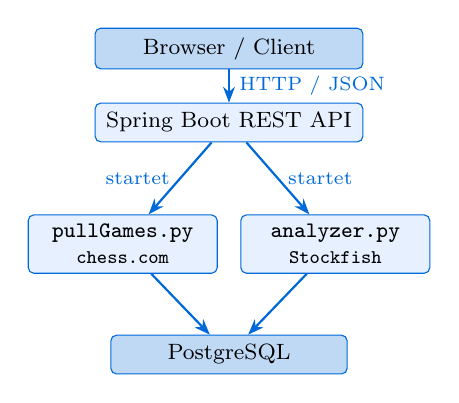
\begin{tikzpicture}[
      box/.style={draw=chessblue, fill=chesslight, rounded corners=2pt,
                  minimum width=3.4cm, minimum height=1.4em, align=center,
                  font=\footnotesize},
      side/.style={box, minimum width=2.4cm},
      db/.style={box, minimum width=3.0cm, fill=chessblue!25},
      arrow/.style={-{Stealth[length=2mm]}, thick, chessblue}
    ]
    \node[box, fill=chessblue!25] (client) {Browser / Client};
    \node[box, below=1.2em of client] (api) {Spring Boot REST API};
    \node[side, below=2.6em of api, xshift=-1.35cm] (pull) {\texttt{pullGames.py}\\ \scriptsize\texttt{chess.com}};
    \node[side, below=2.6em of api, xshift=1.35cm] (ana) {\texttt{analyzer.py}\\ \scriptsize\texttt{Stockfish}};
    \node[db, below=2.2em of $(pull.south)!0.5!(ana.south)$] (db) {PostgreSQL};

    \draw[arrow] (client) -- node[right]{\scriptsize HTTP / JSON} (api);
    \draw[arrow] (api) -- node[left]{\scriptsize startet} (pull);
    \draw[arrow] (api) -- node[right]{\scriptsize startet} (ana);
    \draw[arrow] (pull) -- (db);
    \draw[arrow] (ana) -- (db);
  \end{tikzpicture}
  \end{center}

  \begin{itemize}
    \item Java startet die Skripte \emph{on demand} -- keine Dauer-Services
    \item Logs \& Fehler in getrennte Dateien
  \end{itemize}
\end{frame}

% ---------------------------------------------------------------
\begin{frame}{Spiel-Import}
  \begin{itemize}
    \item \texttt{POST /dispatch/refresh} (Antwort: \texttt{202})
    \item Java startet \texttt{pullGames.py}
    \item holt die letzten 2 Monate von der chess.com API
    \item parst das PGN zu einzelnen Zügen (\texttt{python-chess})
    \item \texttt{Upsert} Spieler + Insert Partie
    \item stoppt an bereits bekannten Partien
  \end{itemize}
\end{frame}

% ---------------------------------------------------------------
\begin{frame}{Stockfish-Analyse}
  \begin{itemize}
    \item \texttt{POST /games/\{id\}/analysis-request} -- markiert
          \texttt{analysisRequested}
    \item \texttt{POST /dispatch/analysis} (Antwort: \texttt{202})
    \item Java startet \texttt{analyzer.py} -- analysiert \textbf{alle markierten Partien}
    \item pro Zug: \textbf{best move} + Evaluation der Engine
    \item \texttt{evalDiff} = Engine-Bewertung vs.\ gespielter Zug
    \item Ergebnis als \texttt{MoveEvaluation} gespeichert
  \end{itemize}
  \begin{block}{Interpretation}
    großer \texttt{evalDiff} $\Rightarrow$ besseren Zug verpasst $\Rightarrow$ Blunder
  \end{block}
\end{frame}

% ---------------------------------------------------------------
\begin{frame}{REST API}
  \begin{center}
  \begin{tabular}{lll}
    \toprule
    \textbf{Methode} & \textbf{Endpoint} & \textbf{Beschreibung} \\
    \midrule
    GET & \texttt{/games} & alle Partien \\
    GET & \texttt{/games/\{id\}} & Partie inkl.\ Analyse \\
    GET & \texttt{/games/users} & alle Spieler \\
    GET & \texttt{/games/count} & Anzahl Partien \\
    POST & \texttt{/games/\{id\}/analysis-request} & Partie für Analyse markieren \\
    POST & \texttt{/dispatch/refresh} & Python-Import starten (\texttt{202}) \\
    POST & \texttt{/dispatch/analysis} & Python-Analyse starten (\texttt{202}) \\
    \bottomrule
  \end{tabular}
  \end{center}
\end{frame}

% ---------------------------------------------------------------
\begin{frame}{Datenmodell}
  \begin{center}
  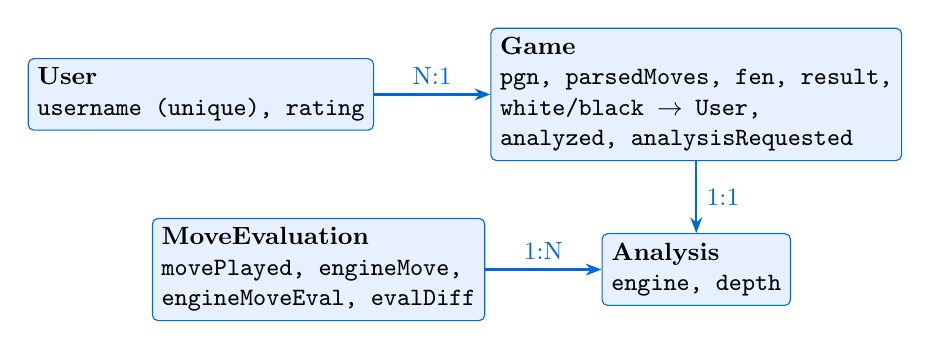
\begin{tikzpicture}[
      node distance=2.6em and 4.2em,
      ent/.style={draw=chessblue, rounded corners=2pt, font=\small, align=left,
                  fill=chesslight},
      arrow/.style={-{Stealth[length=2mm]}, thick, chessblue}
    ]
    \node[ent] (user) { \textbf{User} \\
      \texttt{username (unique), rating} };
    \node[ent, right=of user] (game) { \textbf{Game} \\
      \texttt{pgn, parsedMoves, fen, result,} \\
      \texttt{white/black $\rightarrow$ User,} \\
      \texttt{analyzed, analysisRequested} };
    \node[ent, below=of game] (analysis) { \textbf{Analysis} \\
      \texttt{engine, depth} };
    \node[ent, left=of analysis] (move) { \textbf{MoveEvaluation} \\
      \texttt{movePlayed, engineMove,} \\
      \texttt{engineMoveEval, evalDiff} };

    \draw[arrow] (user) -- node[above]{\small N:1} (game);
    \draw[arrow] (game.south) -- node[right]{\small 1:1} (analysis.north);
    \draw[arrow] (move.east) -- node[above]{\small 1:N} (analysis.west);
  \end{tikzpicture}
  \end{center}
\end{frame}

% ---------------------------------------------------------------
\begin{frame}{Wohin das führt}
  \begin{itemize}
    \item Meine verpassten Züge stecken bereits im \texttt{evalDiff}
    \item Ideen daraus:
      \begin{itemize}
        \item aus Fehlern \textbf{Puzzles} bauen
              („hättest du den Zug gefunden?“)
        \item \textbf{Eröffnungs-Trainer} aus meinen eigenen Partien
        \item sich wiederholende \textbf{Fehlermuster} erkennen
        \item Fortschritt über \textbf{Analysen pro Monat} messen
      \end{itemize}
  \end{itemize}
  \begin{block}{Kernaussage}
    Die Daten liegen schon da -- die Algorithmen obendrauf sind der nächste Schritt.
  \end{block}
\end{frame}

% ---------------------------------------------------------------
\begin{frame}
  \centering
  {\Huge\bfseries Vielen Dank!}
  \vspace{1.5em}

  Fragen gerne an mich.
\end{frame}

\end{document}
